\section{Bottom friction}
%

% - Purpose & Problem description:
%     These first two parts give reader short details about the test case,
%     the physical phenomena involved and specify how the numerical solution will be validated
%
\subsection{Purpose}
%
This test case aims at testing the effect of friction coefficients used in Tomawac, one acting upon energy whereas the other one acts upon the mean directional frequency. This test case is an inheritage of a comparison between Cowadis and Tomawac. There is no measure to validate the test, it is only a non regression testing.



%
\subsection{Description of the problem}
The waves are let freely propagate in a large body of water. The swell should loose some energy and its frequency should change only under the effect of friction bottom (the boundary conditions may be ignored because the domain is very wide).

The expression that is used for computing the friction in Tomawac is as follows :
\begin{equation}
Q_{bf}(\theta,\omega)=-\Gamma \left(\frac{\sigma}{g.\sinh(kd)}\right)F(\theta,\omega)
\end{equation}
Where $\Gamma$, the \telkey{BOTTOM FRICTION COEFFICIENT}, is taken equal to 0.038, its default value.

\subsection{Geometry and mesh}
The computational domain is a 100~km by 25~km rectangle and the flat bottom elevation is taken equal to 5m.

The mesh is made with 492 nodes (80 on the boundary) and 902 triangles.

\begin{figure} [!h]
\centering
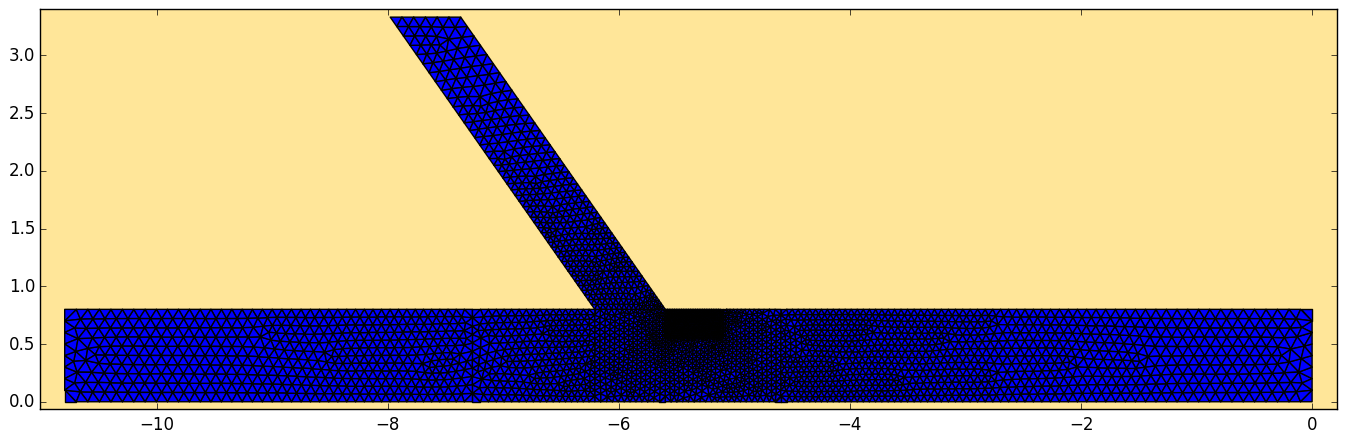
\includegraphics[scale = 0.65]{../mesh.png}
 \caption{mesh of the domain}\label{mailbf}
\end{figure}

% - Physical parameters:
%     This part specifies the geometry, details all the physical parameters
%     used to describe both porous media (soil model in particularly) and
%     solute characteristics (dispersion/diffusion coefficients, soil <=> pollutant interactions...)
%
\subsection{Numerical parameters}
%
Time duration is 30000~s, time step is equal to 100~s, the spectro-angular mesh has 24 angles and 25 frequences spread on a geometric progression common ratio 1.1 with a minimum of 0.056447393.

\subsection{Initial and Boundary Conditions}
%
For both conditions, we take a Jonswap spectrum with a 1~m significant wave heigth, a pic frequency of 0.1 The angular distribution function follows a $\cos^{2s} \theta$ distribution with an angular spreading of 6 and a mean direction of 0.

\subsection{Numerical parameters}


% - Results:
%     We comment in this part the numerical results against the reference ones,
%     giving understanding keys and making assumptions when necessary.
%
%
\subsection{Results}
In this case we just verify that we still have the same results as the ones obtained during the comparison with Cowadis \cite{cowadis}.
\begin{figure} [!h]
\centering
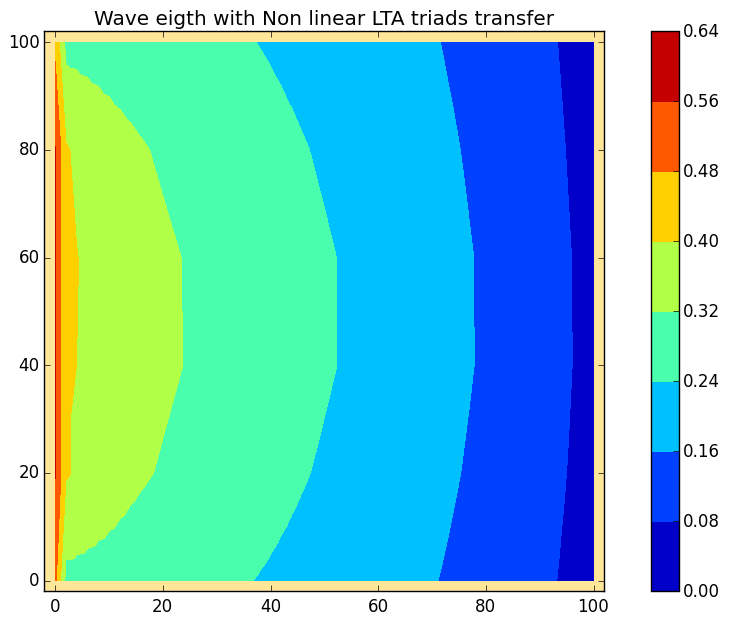
\includegraphics[scale = 0.65]{../results.png}
 \caption{WAVE HEIGHT HM0}\label{mailbf}
\end{figure}
